\documentclass[11pt,a4paper]{jarticle}
\usepackage[dvipdfmx]{graphicx}
\usepackage{url}

\renewcommand{\baselinestretch}{1.05} 
\marginparwidth=0cm
\topmargin=-1cm
\headheight=0.3cm
\headsep=0.7cm
\oddsidemargin=0cm
\evensidemargin=0cm
%\textwidth=43zw
\textwidth=15.92cm
%\textheight=43.3\baselineskip
\baselineskip = 0.5744cm
\textheight=43\baselineskip

\itemsep=0.05\baselineskip
\parsep=0pt
\topsep=0.01\baselineskip
\partopsep=0pt
\listparindent=0zw

%% header and footer
\usepackage{fancyhdr}
\pagestyle{fancy}
\lhead{2014年度 春学期授業}
\chead{インタラクティブ・アート実習}
\rhead{担当教員: 松下 光範}
\cfoot{\thepage}
\renewcommand{\headrulewidth}{0pt}
\renewcommand{\footrulewidth}{0pt}

\usepackage{ascmac}
\usepackage{listings,jlisting}
\usepackage{color}
\definecolor{OliveGreen}{cmyk}{0.64,0,0.95,0.40}
\definecolor{colFunc}{rgb}{1,0.07,0.54}
\definecolor{CadetBlue}{cmyk}{0.62,0.57,0.23,0}
\definecolor{Brown}{cmyk}{0,0.81,1,0.60}
\definecolor{colID}{rgb}{0.63,0.44,0}
\definecolor{rulesepcolor}{gray}{0.666}
\lstset{
  language=Java,%プログラミング言語によって変える。
  basicstyle={\ttfamily\small},
  keywordstyle={\color{OliveGreen}},
  %[2][3]はプログラミング言語によってあったり、なかったり
  keywordstyle={[2]\color{colFunc}},
  keywordstyle={[3]\color{CadetBlue}},%
  commentstyle={\color{Brown}},
  %identifierstyle={\color{colID}},
  stringstyle=\color{blue},
  tabsize=2,
  %frame=trBL,
  %numbers=left,
  numberstyle={\ttfamily\small},
  breaklines=true,%折り返し
  %backgroundcolor={\color[gray]{.95}},
  framexleftmargin=0mm,
  frame=single,
  rulesepcolor=\color{rulesepcolor},
  captionpos=b
}


%%%%%%%%%%%%%%%%%%%%%%%%%%%%%%%%%%%%%%%%%%%%%%%%%%%%%%%%%%%%%%%%
\begin{document}

% title
% \section*{\LARGE{第2講 プログラムと I/O モジュールを組み合わせる}}
\section*{\LARGE{第2講 プログラミングでLEDを制御する}}
Processing と Arduino を接続し LED を制御する。
スイッチの ON/OFF を取得する。

%%%%%%%%%%%%%%%%%%%%%%%%%%%%%%%%%%%%%%%%%%%%%%%%%%%%%%%%%%%%%%%%


\section{Arduino の準備}
本実習ではスイッチやセンサ、LED などを PC から制御するために Arduino\footnote{\url{http://arduino.cc}} というマイコンを用います。

\begin{itemize}
 \item Arduino IDE のインストール
 \item Arduino ドライバのインストール
 \item Arduino に Firmata を書き込む
 \item Firmata の動作確認
 \item Processing に Arduino ライブラリをインストール       
\end{itemize}


\section{Processing から Arduino を制御する}
本実習では Processing で Arduino を制御します。
今回は Arduino の Digital Output を用いて LED の制御したり、
Digital Input を用いてスイッチの ON/OFF を取得したりします。

まず、Processing から Arduino を用いるための準備をしましょう。
\begin{lstlisting}
 import processing.serial.*;
 import cc.arduino.*;

 Arduino arduino;

 void setup() {
   // Arduino.list()[0] は環境によって変える
   arduino = new Arduino(this, Arduino.list()[0], 57600);
 }
\end{lstlisting}
これらの命令は今後も Arduino を用いる際に必ず使うので忘れないように。

\begin{itembox}{Tips}
 COMポート指定についてほげほげ書く
\end{itembox}

\subsection*{LED を点滅させる}
Digital Output を使って LED を点滅させてみましょう。

\subsubsection*{Digital Output}
\begin{itemize}
 \item Digital Output の説明
 \item arduino.pinMode(ledPin, Arduino.OUTPUT);
 \item arduino.digitalWrite(ledPin, Arduino.HIGH);
\end{itemize}

\begin{lstlisting}
import processing.serial.*;
import cc.arduino.*;
 
Arduino arduino;
int ledPin = 13;
 
void setup() {
  size(400, 300);
  arduino = new Arduino(this, Arduino.list()[0], 57600);
  arduino.pinMode(ledPin, Arduino.OUTPUT);
}
 
void draw() {
  arduino.digitalWrite(ledPin, Arduino.HIGH);
  delay(500);
  
  arduino.digitalWrite(ledPin, Arduino.LOW);
  delay(500);  
}
\end{lstlisting}


\subsection*{スイッチの ON/OFF を読み取る}

\subsubsection*{プルアップ/プルダウン抵抗}
プルアップ/プルダウン抵抗についてのせつめいほげほげ

\begin{figure}[h]
 \begin{minipage}{0.5\columnwidth}
  \centering
  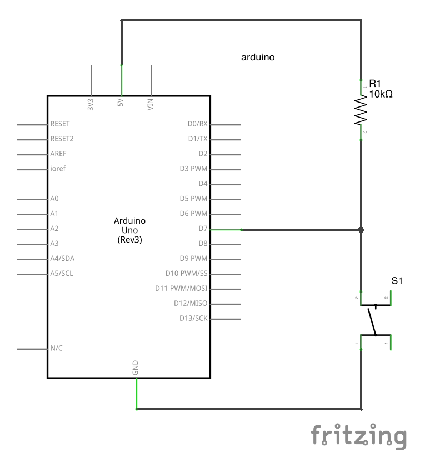
\includegraphics[width=0.8\columnwidth]{img/pullup.eps}
  \caption{プルアップ抵抗}
 \end{minipage}
 \begin{minipage}{0.5\columnwidth}
  \centering
  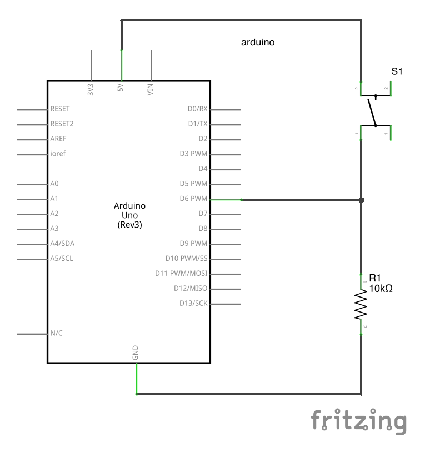
\includegraphics[width=0.8\columnwidth]{img/pulldown.eps}
  \caption{プルダウン抵抗}
 \end{minipage}
\end{figure}

\subsubsection*{Digital Input}
\begin{itemize}
 \item Digital Input の説明
 \item arduino.pinMode(switchPin, Arduino.INPUT);  
 \item arduino.digitalRead(switchPin)
\end{itemize}

\begin{lstlisting}
import processing.serial.*;
import cc.arduino.*;

Arduino arduino;
int switchPin = 8;
 
void setup() {
  size(400, 300);
  arduino = new Arduino(this, Arduino.list()[0], 57600);
  arduino.pinMode(switchPin, Arduino.INPUT);  
}
 
void draw() {
  if (arduino.digitalRead(switchPin) == Arduino.HIGH) {
    background(255, 0, 0);
  } else {
    background(0, 0, 0);
  }
}
\end{lstlisting}



\subsection*{スイッチを押すと LED が点灯するようにする}
上 2 つの合わせ技。

\begin{lstlisting}
import processing.serial.*;
import cc.arduino.*;

Arduino arduino;
int ledPin = 13;
int switchPin = 8;
 
void setup() {
  size(400, 300);
  arduino = new Arduino(this, Arduino.list()[0], 57600);
  arduino.pinMode(switchPin, Arduino.INPUT);
  arduino.pinMode(ledPin, Arduino.OUTPUT);
}
 
void draw() {
  if (arduino.digitalRead(switchPin) == Arduino.HIGH) {
    background(255, 0, 0);
    arduino.digitalWrite(ledPin, Arduino.HIGH);
  } else {
    background(0, 0, 0);
    arduino.digitalWrite(ledPin, Arduino.LOW);
  }
}
\end{lstlisting}

これで入力と出力の両方が実現できました。


\end{document}